\documentclass[xcolor=dvipsnames]{beamer}
\usetheme{Warsaw} % Beamer Theme
\usecolortheme[named=Mahogany] {structure}% Beamer
%%%%%%%%%%%%%%%%%%%%%%%%%%%%%%%%%%%%%%%%%%%%%%%%%%%%%%%%
\usepackage[spanish]{babel}
\usepackage[utf8]{inputenc}      
\usepackage[T1]{fontenc}
\usepackage{lmodern}
\usepackage{amsmath}
\usepackage{amssymb}
\usepackage{hyperref}
\usepackage{tikz}
\newtheorem{Def}{Definición}
\newtheorem{Pro}{Proposición}
\newtheorem{Ob}{Objetivo}

%%%%%%%%%%%%%%%%%%%%%%%%%%%%%%%%%%%%%%%%%%%%%%%%%%%%%%%%%%
\decimalpoint
\AtBeginSection[] {
  \begin{frame}<beamer>
    \frametitle{Contenido}
    \tableofcontents[sectionstyle=show/hide,subsectionstyle=show/show/hide]
  \end{frame}
}
\title[Nombre de la institución]{Título de la presentación}
\vskip 2mm
\author[Nom abrev de la inst]{Nombre del ponente}
\vskip 3mm
\institute[]{Nombre de la institución}
\vskip 3mm
\date{00 de Mes Año}
%##########################################################
\begin{document}
\frame{\titlepage}
\frame{\frametitle{Contenido}\small{\tableofcontents[hideallsubsections]}}
%%%%%%%%%%%%%%%%%%%%%%%%%%%%%%%%%%%%%%%%%%%%%%%%%%%%%%%%%%
\section{Mi primer sección: Introducción}
%%%%%%%%%%%%%%%%%%%%%%%%%%%%%%%%%%%%%%%%%%%%%%%%%%%%%%%%%%
\begin{frame}{Definición}

Contenido ..... 

\end{frame}
%%%%%%%%%%%%%%%%%%%%%%%%%%%%%%%%%%%%%%%%%%%%%%%%%%%%%%%%%%
\begin{frame}{Continuación ...}

Contenido aquí....

\end{frame}
%%%%%%%%%%%%%%%%%%%%%%%%%%%%%%%%%%%%%%%%%%%%%%%%%%%
\section{Mi segunda sección: Desarrollo}
%%%%%%%%%%%%%%%%%%%%%%%%%%%%%%%%%%%%%%%%%%%%%%%%%%%%%%%%%%
\begin{frame}{Incluyendo una imagen}

\begin{figure}
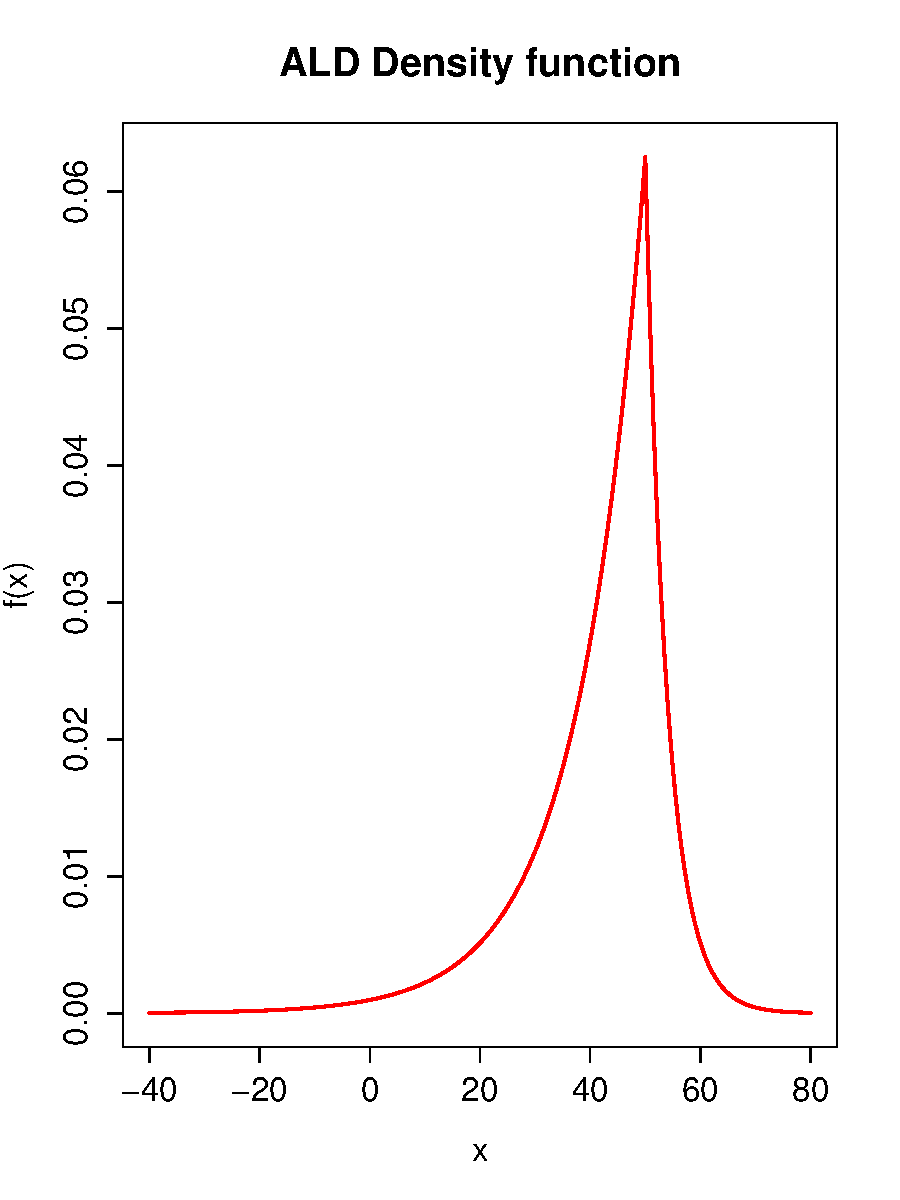
\includegraphics[scale=0.42]{fig1}
\end{figure}

\end{frame}

%%%%%%%%%%%%%%%%%%%%%%%%%%%%%%%%%%%%%%%%%%%%%%%%%%%%%%%%%%
%%%%%%%%%%%%%%%%%%%%%%%%%%%%%%%%%%%%%%%%%%%%%%%%%%%%%%%%%%
\begin{frame}{Ejemplo de Items}


\begin{itemize}
\item Mi primer punto es ....
\item Mi segundo punto es
\end{itemize}



\end{frame}
%%%%%%%%%%%%%%%%%%%%%%%%%%%%%%%%%%%%%%%%%%%%%%%%%%%%%%%%%%%%%%%%%%%%%%%%%%%%%%%%%%%%%%%%%%%%%%%%%
%%%%%%%%%%%%%%%%%%%%%%%%%%%%%%%%%%%%%%%%%%%%%%%%%%%%%%%%%%
\begin{frame}{Mi tema...}





\end{frame}
%%%%%%%%%%%%%%%%%%%%%%%%%%%%%%%%%%%%%%%%%%%%%%%%%%%%%%%%%%
\begin{frame}{Bibliografía}
\begin{thebibliography}{2}

\beamertemplatebookbibitems
\bibitem{pag1} Galarza, C. E.,  Lachos, V. H. (2015). ald:  An R Package for  Asymmetric Laplace Distribution.
\bibitem{pag2} Kotz, S., Kozubowski, T. J., Podgórski, K. (2001). The Laplace Distribution and Generalizations. Birkhäuser, Berlin.
\bibitem{pag3} Yu, K.,  Zhang, J. (2005). A three-parameter asymmetric Laplace distribution and its extension. Communications in Statistics-Theory and Methods, 34(9-10), 1867-1879.
\end{thebibliography}
\end{frame}
%%%%%%%%%%%%%%%%%%%%%%%%%%%%%%%%%%%%%%%%%%%%%%%%%%%%%%%%%%
\begin{frame}

\begin{center}
    \huge{Gracias por su atención}
\end{center}


\end{frame}
%%%%%%%%%%%%%%%%%%%%%%%%%%%%%%%%%%%%%%%%%%%%%%%%%%%%%%%%%%
\end{document}